 \begin{center}
  \textbf{1-ое занятие по алгоритмам.} 
 \end{center}

 \textbf{Поток(flow).} Это математический объект. Мы можем рассматривать как водопроводную сеть, которая представлена в виде взвешенного ориентированного графа. В графе есть две(может больше) особенные вершины - исток и сток. Мы хотим "перегонять" как можно больше воды в секунду.

 \textbf{Сеть} - это ориентированный граф. $с: E \to \mathbb{R} $ - пропускная способность, $e \in V$ - исток,\break$t \in V$ - сток.

  \textbf{Поток} - это функция $f: E \to \mathbb{R} $ которая возвращает поток по ребру. В котором выполняется два правила. (1) Сумма входящей воды равна выходящей. (2) По ребру проходит воды не больше чем его пропускная способность.

  \textbf{Величина потока.} $|f|_t = $ сумма входящих в сток минус сумма всех исходящих из стока.  $|f|_s = $ сумма выходящих из истока минус сумма всех входящих из истока. На самом деле эти суммы равны, доказательство заключается в том что в каждую вершину входит столько же воды сколько и выходит, но в исток "свыше" приходит вода, значит она куда-то должна деться, очевидно что только в сток.

\textbf{Доказательство существования максимального потока.} У потоков есть точная верхняя грань, возьмем последовательность потоков подходящей к точной верхней грани. Выберем какое-то ребро и возьмем бесконечную сходящуюся подпоследовательность из нашей последовательности для ребра. Проделаем данную операцию для каждого ребра, возьмем предел для каждого ребра, все свойства будут выполняться.

Просто искать пути и заполнять их - нельзя. Есть пример даже без циклов, если мы выбрали путь, который блокирует другие пути.

\begin{center}
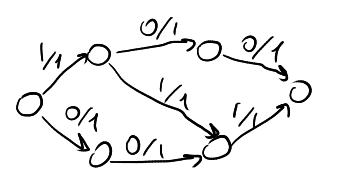
\includegraphics{img1.png}
\end{center}

\textbf{Опр.} Пусть есть сеть и поток, тогда остаточной сетью назовем сеть в которой пропускную способность заменим на (пропускную способность минус поток) и добавим обратное ребро с весом потока.

\textbf{Утв.} Если в остаточной сети есть путь по не нулевым ребрам, то поток не максимален.
